
\section{Introduction}
\label{Introduction}

The High Threshold \v Cerenkov Counter (HTCC) is one of 
the major components of the CLAS12 spectrometer. It 
will be used for electron identification in all experiments 
with electron beams. In combination with the Low Threshold 
\v Cerenkov Counter (LTCC) it will make possible the
identification of charged $\pi$-mesons  over the entire
momentum range up to a maximum of  5 GeV$^2$/c$^2$. 
An overall view 
of the CLAS12 spectrometer is given in Figure~\ref{CLAS12}. Part 
of the infrastructure in the Hall B experimental area and other 
equipment are shown as well.

\begin{figure}
\begin{center}
%\epsfig{file=pictures/FIG1_1_1.eps,width=7cm,angle=-90}
\caption{CLAS12 spectrometer in the experimental Hall B. In light 
green is shown Torus Magnet, Central Detector and HTCC are mounted 
on the extension of Level I of the Main Frame}
\end{center}
\label{CLAS12}
\end{figure}
   
The HTCC is located between the Central and Forward Detectors of 
CLAS12, and mounted on a separate cart that can be moved along 
beam direction. 
 
The radiating gas for the HTCC is CO$_{2}$ gas at  room temperature and 
pressure. The threshold of the detection of charged $\pi$-mesons is 4.9GeV/c, 
and in the entire momentum range below the threshold the rejection factor 
for pions is greater then 2000. The optical  configuration  in the HTCC
is chosen to be similar to LTCC currently used in CLAS. However, 
since the detector is positioned upstream of the drift chambers, it was
decided to use the reflection from  mirror per module, as opposed to
two for the LTCC. The current design comprises 96 light reflection 
and collection modules.

The main working parameters of the HTCC are given bellow:

\begin{center}
\begin{tabular}{|c|c|}
 \hline
\bf Channels & \bf 96 (6 sectors of (2$\times$8) channels each) \\ \hline
\bf Working Gas     & \bf CO$_{2}$\@1atm\@room temperature \\ \hline
\bf Mirror Type & \bf Ellipsoidal, 96 segments  \\ \hline
\bf Photomultipliers & \bf XP4508 (5$''$, Quartz face plate) \\ \hline
\bf Threshold & \bf  4.9GeV/c ($\pi$-mesons) \\ \hline
\bf Rejection Factor & \bf  $>$ 2000\@ p $<$ 4.9GeV/c \\ \hline
\end{tabular}
\end{center}

The overall performance requirements and scope of primary problems
which need to be solved are shown in the following table:

\begin{center}
\begin{tabular}{|p{0.3\textwidth}|p{0.65\textwidth}|}
 \hline
Performance Requirement & Regarding R\&D tasks to be addressed \\ \hline
 \centering \bf High electron detection efficiency  & \bf Development of a technology providing highest finish of mirror surfaces at low cost \\ \hline 
 \centering \bf Run at luminosity $\geq 10^{35}$ cm$^{2}$$\times$sec & \bf Flexibility in distributing angular acceptance over adjacent channels \\ \hline
 \centering \bf Acceptance $\Delta\phi = 2\pi$ in angular range $5^{o} \leq \theta \leq 35^{o}$�& \bf Designing mirrors with no support/alignment parts within acceptance. No dead zones between mirror segments \\ \hline
 \centering \bf Total Thickness $\leq$ 200mg/cm$^{2}$ & \bf Developing technology of mirror construction using materials of low density at no residual stress \\ \hline
\begin{center} \bf Reliability \end{center}& \bf Maintenance free mirror. PMTs, other components (such as HV dividers, Winston Cones, magnetic shields) can be reached and replaced if necessary in situ \\ \hline
\end{tabular}
\end{center}



\subsection{Optical Requirements}
\label{Optical Requirements}

The upgraded CLAS12 spectrometer incorporates several major components 
inherited from CLAS such as the Forward  Time-of-Flight Counters, 
the Low Threshold \v Cerenkov Counter, and Forward Electromagnetic 
Calorimeter. 
It will bebuilt build in the same experimental area. This places  
constraints on the overall CLAS12 design and consequently on all 
detector components while requiring  most efficient acceptance 
coverage.

The HTCC occupies very limited space downstream of the Central Detector
and is mounted between the Microstrip Silicon Tracker and Region I drift 
chambers. Figure~\ref{geometry} illustrates the basic optics of the detector, 
and Figure~\ref{2dview} shows a 3-dimensional view of themirror and 
PMTs for one sector.
The design is such that that the photons are reflected only once by one 
of the elliptical mirrors and then directly impinge on the photocathode 
of photomultiplier tube. However, since the optical design must be  forgiving 
in the sense that the light collection efficiency  
must be relatively insensitivesensitive to target length and position, 
smearing of photon distribution due to the influence of the
magnetic fields of the Central Solenoid on the particle trajectories,
the  photomultiplier tubes are equipped with {\it Winston} light collection cones. 

\begin{figure}[ht]
\begin{center}
%\framebox{\epsfig{file=pictures/FIG2_1_1.eps,width=7cm,angle=-90}}
\caption{Geometry and main parameters of HTCC}
\end{center}
\label{geometry}
\end{figure}

\begin{figure}
\begin{center}
%\epsfig{file=pictures/FIG2_1_2.eps,width=7cm,angle=-90}
\caption{3D-view of mirror and PMTs for one sector}
\end{center}
\label{2dview}
\end{figure}

The optical properties of the mirrors, Winston cones and photomultiplier 
tubes are optimized for maximum reflection and detection of the \v Cerenkov 
light.Since much of the \v Cerenkov light is in the ultra violet (UV), 
the working surfaces of mirrors and cones will consist of evaporated
coatings of aluminum, which has a high reflectivity from the near UV through
the visible wavelength regions. An evaporated   magnesium fluoride (MgF$_{2}$) 
protective coating will be provided to prevent oxidation of the aluminum, while
transmitting light through the required wavelength range. 
The  photomultiplier tubes (PMT)consists of the Photonis XP4508 
with quartz face plates, again, to maximize efficiency in the UV ramge. 
 
\subsection{Physical Environment} 
\label{Physical Environment}

 The HTCC is a single module detector covering all six sectors for scattering 
angles in the  range  $\theta = 5^\circ$  to $37^\circ$
in the entire $\Delta\varphi = 2\pi$ range. Since the Detector is a single
unit it can be moved alongthe  beam direction or 
removed from the beam if necessary. It is located in a strong magnetic field 
of the superconducting solenoid of the Central Detector. The light collection 
geometry of the HTCC is such that all 96 photomultiplier tubes are located in 
the fringe field domain at radial distances of 124.5cm or greater from 
the electron beam. These distances are chosen to be maximal
while still small enough to fit in the Hall B main frame infrastructure 
(Figure~\ref{htcc}) and to allow moving the detector upstream for 
CLAS12 alignment and maintenance purposes.

\begin{figure}
\begin{center}
%\epsfig{file=pictures/FIG2_2_1.eps,width=7cm,angle=-90}
\caption{HTCC and Central Detector (moved upstream under Main Frame)}
\end{center}
\label{htcc}
\end{figure}

The space limittions of the HTCC along the beam direction defines the
intensity of the \v Cerenkov photons expected at a given pressure of working gas.
The design of CLAS12 specifies that the entry window of \v Cerenkov Counter is 
located at $\sim$0.10 cm distance downstream of the SVT of the Central Detector,
and the exit window is 10cm  upstream of the Region 1 drift chambers. That 
leaves distances that scattered electrons travel in the CO$_{2}$ radiator 
$\sim$ 131 cm at $\theta = 5^\circ$ and $\sim$ 181 cm at  $\theta = 35^\circ$.
The geometry of the HTCC is optimized to keep difference in path lengths minimal.
The distribution of magnetic fringe field were
taken into consideration in  locating the PMTs. The detailed optical geomentry
and estimated signal strength is discussed in detail later in Section XXX.

The intrinsic angular and momentum resolutions of CLAS12 along with its 
capability of running at high luminosities puts serious constraints on 
both the thicknesses and materials that can be used in HTCC mirrors. 
These limitations on materials and estimates of required and achievable 
thicknesses are given in Section XXX.
 
 Another constraint  comes from the 
acceptance specifications for Regions 1, 2 and 3 (R1,R2 and R3 respectively)
drift chambers which are located  downstream of the HTCC. The polar angle 
acceptance for the drift chambers  $\theta = 5^\circ $ to $44^\circ$ 
is greater than for the HTCC. The support structure for the eliptical
mirrors has to be located in the relatively narrow {\it shadow} region 
of the the coil planes of CLAS12 Torus Magnet, and the mirror substrate
support built of light materials possible.
 

%here

\subsection{Overall design}
\label{Overall design}

The overall approach to working out  HTCC design is a twofold task,
first to outline general demands on the  HTCC  performance and then 
define ranges for critical parameters of the major componants
such  elliptical mirrors.

The main requirements are:
\begin{itemize}
\item High electron detection efficiency, low background
\item Capability of running at luminosity  ${\cal L} \geq 10^{35} cm^{-2} \times sec^{-1}$
\item Angular acceptance $5^{o}�\leq \theta \leq 35^{o}$� and $\Delta \varphi \approx 2 \pi$
\item Lightweight, as less material as possible within acceptance to meet the expected angular and momentum resolutions of CLAS12, -- $\delta \theta \leq 1.5$~mrad,  $\delta \varphi \leq 5$~mrad, and $\Delta p/p \leq 1\% 
$
\end{itemize}

  The view of HTCC is given in Figure~\ref{back}.
  
  
  
\begin{figure}
\begin{center}
%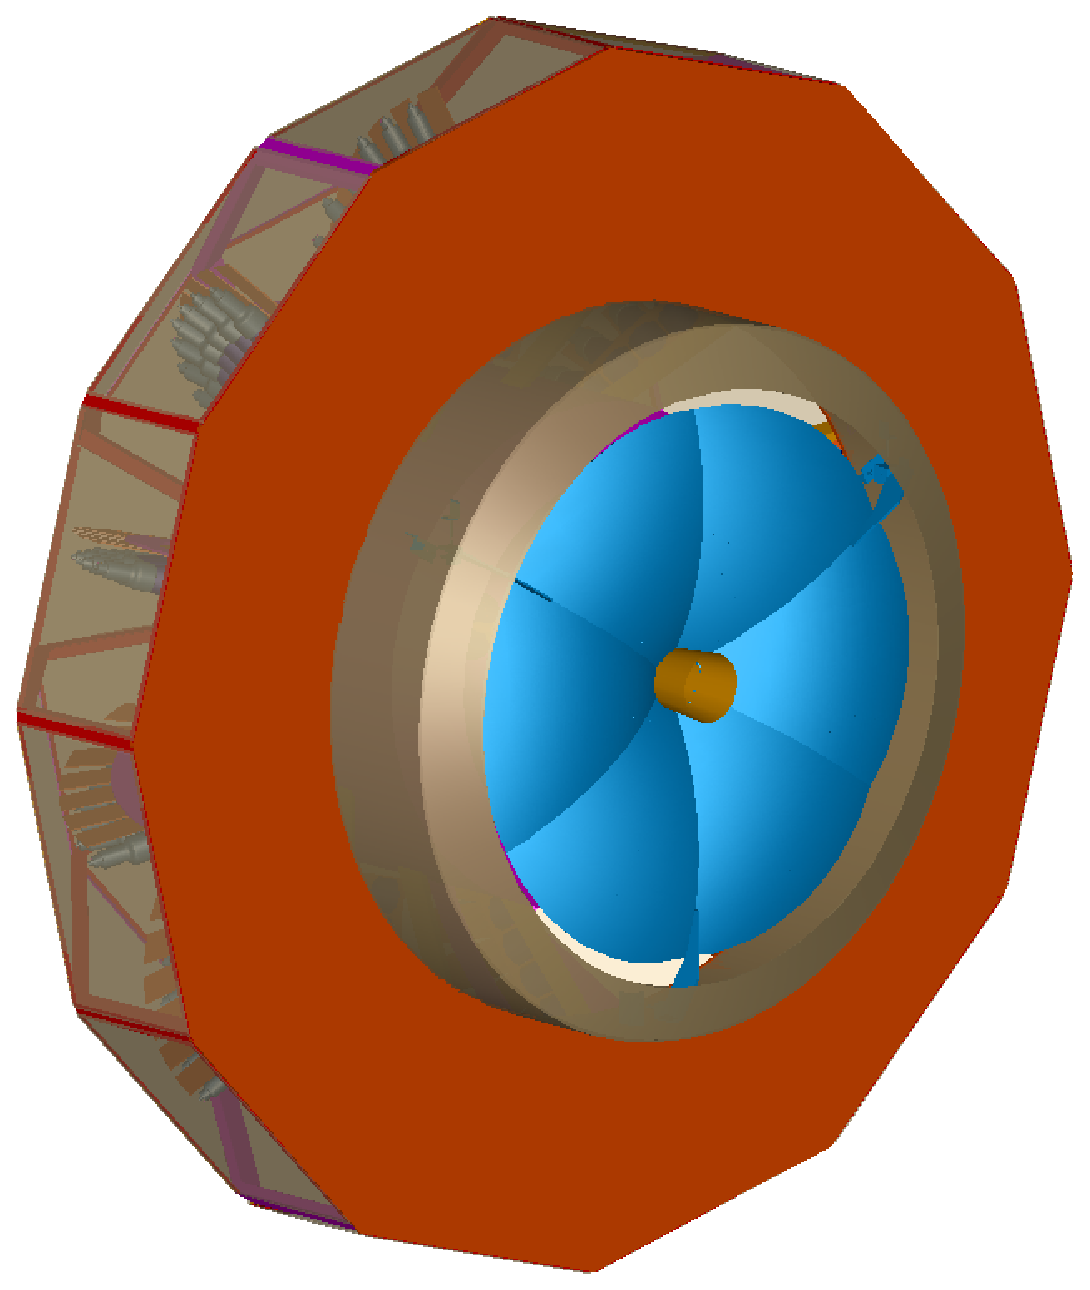
\epsfig{file=pictures/FIG2_3_1.eps,width=7cm}
\caption{Back view of the HTCC, in blue shown Elliptical mirror}
\end{center}
\label{back}
\end{figure} 

 A detailed description of the  current status of the detector design 
is provided in Section  XXX. Some specific features are:
\begin{itemize}
\item Thin entry and exit windows ($\sim$0.6mg/cm$^{2}$ of Polyethylene and $\sim$16mg/cm$^2$ of $\rm ROHACELL$ XF31 foam sheet respectively)
\item Ultra thin self supporting mirror
\item Capability of working with different types of high density M\"oller shields 
\end{itemize}

Total radiation length of the detector is $\sim$1.6\% including contributions 
of CO$_2$ radiator, $\sim$0.8\%, and of the mirror, which does not 
exceed 0.8\%. Since the number of photons per event is proportional to a 
total radiation length of the radiator, the only way to decrease {\it thickness}
of the detector without compromising its performance is to use thinner mirrors
backing.
Figures~\ref{resolution}a,b and c illustrate the changes in CLAS12 resolution
for different mirror thicknesses: standard ($\sim$200mg/cm$^{2}$) and 
reduced to $\sim$100mg/cm$^{2}$.

\begin{figure}
\begin{center}
%\epsfig{file=pictures/FIG2_3_2a.eps,width=5cm,angle=-90}
%\epsfig{file=pictures/FIG2_3_2b.eps,width=5cm,angle=-90}
%\epsfig{file=pictures/FIG2_3_2c.eps,width=5cm,angle=-90}
\end{center}
\caption{a -�momentum, b�- angular, and c -�spatial resolution of CLAS12}
\label{resolution}
\end{figure} 

The results show a relatively small improvements in momentum, angular and 
spatial resolutions for thinner mirrors, indicating that the influence of 
mirror thickness is small or comparable with contributions of other CLAS12 
detector components.

\section{Optical Design and Construction}
\label{Details}

 The most challenging aspect of the HTCC is the construction of the
 elliptical mirror. In addition to being very lightweight and 
self-supportive, there must not be shadowing among adjacent mirrors or gaps 
left between them. This problem has been worked out as follows:

Each mirror surface is an ellipsoid of rotation so the line
of intersection of adjacent  mirror surfaces is curved. If two coplanar 
ellipses intersect, revolving each ellipse about own major axis give
two ellipsoids of rotation, (1) and (2), represented by following equations:
 
 \begin{eqnarray}
 \frac{x^{2}+(y-y_{1})^{2}}{a_{1}^{2}} & + & \frac{(z-z_{1})^{2}}{b_{1}^{2}} = 1  \nonumber\\
 \label{elips}\\
 \frac{x^{2}+(y \cdot cos \theta-z \cdot sin \theta)^{2}}{a_{2}^{2}} & + & \frac{(y \cdot sin \theta-z \cdot cos \theta)^{2}}{b_{2}^{2}} = 1 \nonumber  \end{eqnarray}
where $(y_{1},z_{1})$ are coordinates of center of ellipse (1), $a_{1},a_{2}$ and $b_{1},b_{2}$ respectively are minor and major radiuses of ellipses, $\theta$ is angle between major axis $b_{2}$ and OZ axis in YOZ-plane. Considering the system in $X = c<a_{1}$  plane, we get (assuming $a_{1}<a_{2}$): 
 \begin{eqnarray}
 \frac{(y-y_{1})^{2}}{a_{1}^{2}} & + & \frac{(z-z_{1})^{2}}{b_{1}^{2}} = c_{1}^{2}  \nonumber \\
 \label{elips_var} \\
 \frac{(y \cdot cos \theta-z \cdot sin \theta)^{2}}{a_{2}^{2}} & + & \frac{(y \cdot sin \theta-z \cdot cos \theta)^{2}}{b_{2}^{2}} = c_{2}^{2} \nonumber  \end{eqnarray} 
 
 
By excluding one variable from (\ref{elips_var}) we arrive at a general quartic 
equation :
\begin{equation}
p_{0}z^{4}+p_{1}z^{3}+p_{2}z^{2}+p_{1}z+p_{4}=0
\label{quadrat}
\end{equation} 

which always can be solved, and in the case of the HTCC geometry has 
two roots (see Figure~\ref{figelips}). So, from (\ref{elips_var})  
we obtain two points $P_{1}^{(c)}(y_{1},z_{1})$ and $P_{2}^{(c)}(y_{2},z_{2})$ 
in the plane $X = c$,which satisfy equation (\ref{elips})  as well at $x =c$: 
$P_{1}^{(c)}(c,y_{1},z_{1})$ and $P_{2}^{(c)}(c,y_{2},z_{2})$ are the roots 
of (\ref{elips}). Another two roots of (\ref{elips}) can be found at $x=0$ 
(the YOZ-plane): $P_{3}(0,y_{1},z_{1})$ and $P_{4}(0,y_{2},z_{2})$.
Three out of any four roots define a plane. It can be shown that the remaining 
root  belongs to the same plane as well. Since we arbitrarily used $X = c$, 
all points of intersection (intersection curve) of the two ellipsoids belong
to the same plane. This allows us to  build   mutually self-supporting
elliptical mirrors in which there are no gaps or shadowing of one mirror by 
the next. As a result, the cutting of segments along the perimeter and 
final assembly become relatively simple. Moreover, there will be no shadowing 
of one mirror by another, no "dead" zones for any electrons from 
target within  the acceptance. This also  eliminates need of having a 
support structure for any single mirror segment and consequently makes 
it possible to construct the most efficient and lightweight mirror. 

\begin{figure}
\begin{center}
%\epsfig{file=pictures/FIG2_4_1.eps,width=5cm,angle=-90}
\caption{Ellipses of adjacent mirrors intersecting in two points}
\end{center}
\label{figelips}
\end{figure} 

\begin{figure}
\begin{center}
%\epsfig{file=pictures/FIG2_4_2.eps,width=7cm,angle=-90}
\caption{Planes of intersection of adjacent mirror segments}
\end{center}
\label{planes}
\end{figure} 

Figure~\ref{planes} shows 8 intersecting mirrors forming half of the mirror for 
array for one sector. In the table are given exact coordinates of points
defining planes of intersection between segments and used in corresponding 
MC simulations. Figure~\ref{mirror} illustrates a concept of assembly.
Approximate dimensions in inches of the mirror segments are given in the table.


\begin{figure}
\begin{center}
%\epsfig{file=pictures/FIG2_4_3.eps,width=7cm,angle=-90}
\caption{Elliptical mirror segments cut along planes of intersection. Set of 8 segments cover $1/2$ of the acceptance of one sector. A mirror image of this set covers the other half of the acceptance.}
\end{center}
\label{mirror}
\end{figure} 
                                                                        
Tolerances of construction are critical for the HTCC 
performance. Typical tolerances for cutting substrates are of the order 
(6 of 0.0010 ??? 0.006"?) and are insignificant. So, the expected average
deviation from the nominal geometry would be mostly due to the accuracy that 
can be achievable at the assembly stage. It is anticipated to keep the assembly 
tolerance within (60.0200????) for one mirror segment. Parallel shifts 
will not affect the  light collection because of the large overall acceptance,
whereas unwanted rotation of a segment during assembly might require some 
adjustment of PMT positions. At the given average width of segment,
$\sim$ 5.60 "  (see Figure\ref{mirror}),  the angular equivalent of
( 60.0106 ?????)  is $\sim$ 2 mrad or less. This is the worse possible case 
since all segments except of \#1 are of length greater then 5.60 ".  
The average distance between mirrorx and corresponding PMTs is $\sim$
(80.50????). Therefore the shift of the image in the focal plane of PMT is 
less then 0.150??? ($\sim$ 3.8mm). This estimate is to be examined in
R\&D in 2007. 
									    
\subsection{Mirror Prototyping}
\label{Mirror}
		     
All main features of HTCC and properties of components are planned to be examined
and checked by prototyping of key elements and testing. In this section 
we present results on prototyping of a mirror segment obtained in FY06, and 
describe current R\&D efforts on building a mirror consisting of 3 mirror 
segments.

The main R\&D goal is to find ways of building an elliptical mirror of
\begin{itemize}
\item 200mg/cm$^{2}$ of total thickness
\item minimal residual stress (no adjustment in situ)
\item highest possible finish of working surface
\item reasonable cost
\end{itemize}

 A mirror substrate consists of a thermally shaped plain Mylar film of 
thickness 0.0050",  laminated to an ellipsoidal substrate made of rigid 
polymethacrylimide polymer foam Rohacell HF31 ($\rho \approx 31$mg/cm$^{3}$). 
In the entire  construction procedure the working surface of the Mylar film 
stays untouched throughout all stages. The aluminum reflector and optical 
coating of magnesium fluoride (MgF$_{2}$) will be vacuum deposited onto the 
mylar surface after the the substrate and mylar are joined as a completed unit. 
A set of molding tools is used for shaping of Mylar film into the elipsoidal
shape which mates with the Rohacell substrate without residual stresses.
One of the mold fixtures attached to the bottom plate is shown 
In Figure~\ref{mold} . 
The top surface of the mold is cut  to the exact shape of specified ellipsoid 
of rotation by computer controlled milling using a ball end mill. The thickness 
of film is taken into account. The  top of the mold is then polished  to 
remove scallops left after milling. The Mylar film is shaped by this 
surface, so the finish has to be smooth enough to avoid a {\it telegraph wire}
effect, although the surface does not have to be of mirror quality.  
 
\begin{figure}
\begin{center}
%\epsfig{file=pictures/FIG2_5_1.eps,width=7cm,angle=-90}
\caption{Mold installed on bottom plate}
\end{center}
\label{mold}
\end{figure} 

For better control of the Mylar film edges and to minimize effects of thermal 
contraction a thin aluminum support guard is installed surrounding the mold,
as shown in   Figure~\ref{mold}. There is a small gap of $1/80$" width
left between the support and mold. The support has a profile (shown in red) 
parallel to the edge of ellipsoidal surface of the mold.  The gap is so small 
that the edge of shaped Mylar film is defined not by mold but by support. This 
results in a better alignment of the film with the foam substrate while gluing.


\begin{figure}
\begin{center}
%\epsfig{file=pictures/FIG2_5_2.eps,width=7cm,angle=-90}
\caption{Support installed around mold}
\end{center}
\label{support}
\end{figure}  

In Figure~\ref{vacuum} the wall of the vacuum chamber attached to the bottom 
plate is shown. The wall has high temperature rated vacuum o-rings installed 
both on top and bottom.
 
\begin{figure}
\begin{center}
%\epsfig{file=pictures/FIG2_5_3.eps,width=7cm,angle=-90}
\caption{Vacuum chamber with mold}
\end{center}
\label{vacuum}
\end{figure}  

The height and profile of the top of the wall is cylindrical, such that 
there is approximately constant clearance of $\sim$ 1/40" between this 
surface and ellipsoidal surface of the mold. The inside gap between the wall 
and support is quite wide. It has to be wide enough for the Mylar film to 
concave channels under applied pressure. These channels are formed all the way 
around the support and are necessary for tension relief
when the  chamber is being cooled down and then depressurized.

\begin{figure}
\begin{center}
%\epsfig{file=pictures/FIG2_5_4.eps,width=7cm,angle=-90}
\caption{Vacuum chamber with mold and precut Mylar film}
\end{center}
\label{Mylar}
\end{figure} 

A portion of Mylar film is put on top of the vacuum chamber, as shown 
(in transparent yellow) on Figure~\ref{Mylar}. The top surface of the 
Mylarw remains untouched during cutting and installation of  the film. 
 A flange is placed on the top of the Mylar and tightened down to the wall.
Then the air in the chamber is pumped out so that the Mylar is 
deflected under atmospheric pressure, as in Figure~\ref{Mylar_var}.

 
\begin{figure}
\begin{center}
%\epsfig{file=pictures/FIG2_5_5.eps,width=7cm,angle=-90}
\caption{Vacuum chamber withmold and Mylar film}
\end{center}
\label{Mylar_var}
\end{figure} 

At this point, while still at room temperature, the  Mylar is touching 
the mold, and the area of contact between them is about 60-70\% of maximum. 
To provide a 100\% contact the vacuum chamber is heated inan the oven to
a temperatire of 1708C. During the heating process, which takes about 4 hours,
the chamber remains connected to a vacuum pump running outside the oven. 
To increase the deflection of the unsupported portion of Mylar film (along the
wall) additional pressure is applied to the film. This is done by covering 
the vacuum chamber with a lid installed on the top of flange, as shown in
Figure~\ref{Mylar_pres}.The volume under the lid is then pressurized 
with dry nitrogen.



\begin{figure}
\begin{center}
%\epsfig{file=pictures/FIG2_5_6.eps,width=7cm,angle=-90}
\caption{Vacuum chamber equipped with lid allowing molding of Mylar at higher
pressures}
\end{center}
\label{Mylar_pres}
\end{figure} 


The maximal differential pressure applied to the Mylar can be as high as 
3 Kg/cm$^{2}$. Tested stable results were obtained at differential pressures
in the range  2.0 to 2.55 Kg/cm$^{2}$, depending on temperature. 
The cooling of the chamber back to the room temperature is the last step 
in the thermal shaping. The working differential pressure, once reached,
 is monitored and kept constant during entire cooling cycle. After completion, 
the differential pressure is brought back to atmospheric and lid removed. 
A frame, shown on Figure~\ref{glue}, is glued onto the already shaped
Mylar film. The bottom surface of the frame has the required ellipsoidal shape.
On the top there is a groove cut fora  vacuum o-ring. In the figure
several installed studs are shown in red. Figure~\ref{glue_var} illustrates 
the gluing of the frame onto the pressurized thermally shaped Mylar. 
The largest portion of the Mylar, even while pressurized, is stress free, 
That portion of the surface  which is in full contact  with mold, is leaning 
on it and therefore no stresses are involved here. Only the unsupported
deflected portion of Mylar that is out of the gluing frame is under the stress.
After the glue is polymerized a flat Plexiglas lid is attached to the frame. 
Then the chamber is depressurized. The deflected portion of Mylar provides 
stress relief, shaped at no residual stress. The Mylar film together with frame 
and lid  is cut out as a single  unit for farther use. 


\begin{figure}
\begin{center}
%\epsfig{file=pictures/FIG2_5_7.eps,width=4cm,angle=-90}
\caption{Gluing frame}
\end{center}
\label{glue}
\end{figure} 

\begin{figure}
\begin{center}
%\epsfig{file=pictures/FIG2_5_8.eps,width=7cm,angle=-90}
\caption{Frame glued onto thermally shaped Mylar film leaves Mylar stress free
 after chamber is depressurized.}
\end{center} 
\label{glue_var}
\end{figure}

The other important component of the morror is the mechanical support
substrate, which is made of rigid foam. 
A sheet of polyme of certain size is sanded down, under its 
own weight, until it  providing a flat base. The top of the flat sheet 
is cut by CC milling to the concave ellipsoidal shape, which  mates
to the back surface of the Mylar mirror substrate, as seen in 
Figure~\ref{flatface}. The length and width are appropriate for gluing 
frame and mold.

\begin{figure}
\begin{center}
%\epsfig{file=pictures/FIG2_5_9.eps,width=7cm,angle=-90}
\caption{ Substrate: flat face down, cylindrical top}
\end{center} 
\label{flatface}
\end{figure}

In order to process the front (working) surface, the substrate is mounted on an 
auxiliary table and glued to it along the edges at several locations, as shown 
in Figure~\ref{auxiliar}. The top of the table and back of the substrate have
exactly the same ellipsoidal shape, thus providing the required rigidity 
for further processing.

\begin{figure}
\begin{center}
%\epsfig{file=pictures/FIG2_5_10.eps,width=7cm,angle=-90}
\caption{Substrate mounted on auxiliary table}
\end{center} 
\label{auxiliar}
\end{figure}


Figure~\ref{computer} shows the  cutting of the working surface to the shape 
of an ellipsoid. The ellipsoid parameters were defined by taking into
 account the thickness of the anticipated glue joint and of the thermally 
shaped Mylar film. The diameter of a ball end mill, regime of cutting and value
of overlaying steps  between consequent cuts were optimized to get surface
finish  smooth enough so that any polishing would not be necessary. 
Due to the foam structure there were no scallops observed. In
Figure~\ref{prototype} are shown sample pieces of thermally shaped Mylar films, 
the mold used in shaping them, and completely processed foam substrate mounted
on the auxiliary table.

\begin{figure}
\begin{center}
%\epsfig{file=pictures/FIG2_5_11.eps,width=12cm,angle=-90}
\caption{Computer Controlled cutting of ellipsoidal surface of foam substrate}
\end{center} 
\label{computer}
\end{figure}

\begin{figure}
\begin{center}
%\epsfig{file=pictures/FIG2_5_12.eps,width=12cm,angle=-90}
\caption{Substrate components and metal tooling used in construction of mirror prototype}
\end{center}
\label{prototype}
\end{figure}

The final step in mirror construction is the gluing of the shaped Mylar onto 
the ellipsoidal substrate. The gluing frame, with transparent Plexiglas lid 
on the top, and the Mylar film attached to the bottom is pressurized at 
differential pressure up to $\sim$ 2310$^{-2}$ Torr, so that the film 
bulges out beyond its normal convexity. Low viscosity degassed epoxy glue 
with extended polymerization time is uniformly applied to the ellipsoidal 
surface of the substrate which remains attached to the auxiliary table. 
Then the pressurized frame with bulged Mylar is placed on top of the
substrate slowly enough to let trapped air bubbles escape. A transparent lid 
allows visual control of quality of the joint. The Mylar is fully pressed
 against the substrate, and stays under uniformly distributed pressure 
until the epoxy glue is cured. The position of the frame relative to the table
is controlled as well as the thickness of glue joint. After curing the 
frame is depressurized, the lid removed, the auxiliary table with  
its components is placed back on the CC milling machine. The
inner portion of the composite substrate is directly cut out through 
an opening on the frame. Measurements have shown that the total thickness of 
the composite substrate was 73-74 mg/cm$^{2}$. There is a potential 
of further decreasing a mirror's thickness without altering  the technology 
described in this section. It would leave some contingency in varying 
mirror thickness  within factor of $\sim$ 2 while optimizing the 
overall rigidity.


In 2007 R\&D is planned to check the last step of  construction of the
mirror consisting of three different ellipsoidal segments. 
A critical issue to be addressed is whether the estimated tolerances of 
assembly can be achieved. 


Each of the three mirror segments, once built according to already established 
technology, is put on the modified auxiliary table with special grooves cut 
on top. Then all four sides (one at the time) are cut under particular
angles (all different), defining the orientation of the planes along which 
ellipsoids  intersect. The accuracy of cutting (including positioning) is 
limited typically by (60.0010 ????).  Figure~\ref{compl_cut} shows a 
substrate which has been processed 
on all sides (in yellow)  mounted on the modified auxiliary table.
The sSides of all segments are cut using their own table since the 
angles and dimensions are different for each. But, the back surfaces of 
all three segments, and the top of  corresponding tables are ellipsoidal 
 with the same parameters, so that the segments can be mounted next to each 
other on a larger table ( with top of cylindrical shape????). This is 
illustrated in  Figure~\ref{segments}. After alignment checks they will be 
glued together along the planes of intersection.


\begin{figure}
\begin{center}
%\epsfig{file=pictures/FIG2_5_13.eps,width=12cm,angle=-90}
\caption{Completely cut maunted on the modified auxiliary table}
\end{center}
\label{compl_cut}
\end{figure}

\begin{figure}
\begin{center}
%\epsfig{file=pictures/FIG2_5_14.eps,width=12cm,angle=-90}
\caption{Mirror segments mounted on big table. Left and right sides of mirrors are planes along which will be glued adjacent similar mirror assembly.}
\end{center}
\label{segments}
\end{figure}


\subsection{Light Collection Cones.}
\label{Light Collection}

GEANT simulations of HTCC optics and performance show that for point like target
 with no magnetic field almost all \v Cerenkov photons are focused on photocathod
 of diameter 110mm, which is minimal for 50 PMTs from Photonis. In experiments 
on CLAS12 a standard cryogenic targets are 50mm of length, and in some 
experiments targets as long as up to 100mm can be used. For all experiments 
with electron beam superconductive solenoid and \v Cerenkov counters will be 
used. As it was mentioned in section \ref{Optical Requirements}, to have 
efficient \v Cerenkov light collection for extended targets in magnetic fields
 a light collection cones are necessary. To define main parameters for Winston
 Cones we required an opening diameter of 7.50 and distance from PMT 
photocathode (\&110mm)  to be equal 80 allowing magnetic shields be extended
 far enough beyond photocathode. Direct comparison of such Winston Cone angular 
acceptance with results of MC simulations showed that the Winston Cone�s 
acceptance is much wider, and the opening diameter is big enough to collect 
at least 95\% of \v Cerenkov light in experiments with two possible polarities 
of CLAS12 Torus Magnet without any adjustments of PMTs location or orientation.


There are  well established and experimentally checked technologies for 
constructing Winston Cones. Such light concentrators were built for the existing 
Low Threshold \v Cerenkov Counter of CLAS the electroforming technology
and have revealed maintained undiminished  performance for more than
a decade. The technical specifications and requirements of the proposed Winston 
Cone for the  HTCC, similar of those used in CLAS, are given in Table~ref{HTCC}. 
The corresponding parameters are given in Figure~\ref{Winston}.


\begin{figure}
\begin{center}
%\epsfig{file=pictures/FIG2_6_1.eps,width=10cm,angle=-90}
\caption{Winston Cone for HTCC}
\end{center}
\label{Winston}
\end{figure}


\begin{table}
\centering
\caption{Specifications for HTCC Winston Cones for CLAS12 spectrometer}
\label{HTCC}
\vspace{0.2cm}

\begin{tabular}{|c|c|c|}
\hline
{\bf SPECIFICATION} & {\bf DATE} & {\bf SOURCE}  \\ \hline
Winston Cone Definition&        &             \\ \hline
\begin{minipage}[l]{0.68\textwidth} A Winston Cone is a non-imaging light collector designed to collect light from a range of incident angles on a given circular area and �collect� that light onto a smaller area. The Winston Cone is not a focusing device, but it is highly efficient in collecting light. Its general shape is that of a parabola revolves about an axis of symmetry of the parabola.\end{minipage}  &                                    &            \\ \hline
{\bf BASIC}&  & \\ \hline
\begin{minipage}[l]{0.68\textwidth}
Material = copper outer surface with inner coatings of nickel, aluminum, and magnesium fluoride (see below)
\end{minipage}  &  12/2006                                  &   P. Stoler         \\ \hline
Weight = 4 lbs (approximately) & 12/2006  &Y. Sharabian \\ \hline
Life time = 30 years with no optical degradation & 12/2006  & P. Stoler\\ \hline
Dimensions  = \o7.5$''$$\times$8.0$''$ long & 12/2006 & Y. Sharabian\\ \hline
\begin{minipage}[l]{0.68\textwidth}
Optical and structural properties tolerant to high radiation dose 20 Megarad/20 years
\end{minipage} & 09/1991 & C. Zorn\\ \hline
Most radiation is in x-ray region, some relativistic particles & 05/1992 & C. Zorn\\ \hline
MANUFACTURING & & \\ \hline
Slope errors $<1^{o}$ & 12/2006 & D. Kashy \\ \hline
Surface finish of Root Mean Square = 0.5 $\mu$m (microns) & 12/2006 & Y. Sharabian\\ \hline
\begin{minipage}[c]{0.68\textwidth}
Scratches occurring in forming operation etc. need not be removed provided in the final product there are less than 4/cone and\\ 
\begin{tabular}{cl}
1) & they are less than 2.54 cm in length \\
2) & they are less than 0.15 $\mu$m (microns) deep \\
\end{tabular} \\
Open Ends flat within $0.03''$
\end{minipage} & 12/2006 &Y. Sharabian \\ \hline
{\bf OPTICS} & 12/2006 &Y. Sharabian \\ \hline
{\bf MATERIAL} & 12/2006 & P. Stoler \\ \hline
\begin{minipage}[c]{0.68\textwidth}
Copper: \\
\begin{tabular}{cl}
 &   Thickness = 0.040$''$ nominal \\
 &   Application method = electroformed \\
 &   None-magnetic \\
\end{tabular} \\    
Nickel: \\
\begin{tabular}{cl}
 &   Thickness = 0.0005$''$ nominal \\
 &   Application method = electroformed \\
 &   Allowable magnetic properties \\
\end{tabular} \\ 
Aluminum: \\
\begin{tabular}{cl}
 &   Thickness $\approx$ 0.04 $\mu$m (microns) \\
 &   Application method = vacuum (vapor) deposition \\
 &   None-magnetic \\
\end{tabular} \\ 
Magnesium fluoride (protective coating) \\ 
\begin{tabular}{cl}
 &   Thickness = as required to meet reflectivity specifications \\ 
 &   Application method = vacuum (vapor) deposition) \\
 &    None-magnetic \\
\end{tabular} 
\end{minipage} & & \\ \hline
\end{tabular}
\end{table}
\newpage

\begin{table}
\centering
\begin{tabular}{|c|c|c|}
\hline
\begin{minipage}[l]{0.68\textwidth}
{\bf ENVIRONMENTAL} 
\end{minipage} & 12/2006 & Y. Sharabian \\ \hline
\begin{minipage}[l]{0.68\textwidth}
Operating \@ CO$_{2}$ at 1.001 atmosphere, temperature = 22$^{o}$~C
Stored in plastic bag w/ambient air to avoid dust contamination
DO NOT contact reflective surface with anything
Wash reflective surface w/only optical liquid (Check this spec)
\end{minipage} & & \\ \hline
\end{tabular}
\end{table}

\begin{figure}
\begin{center}
\vspace{2cm}
%\epsfig{file=pictures/FIG2_7_1.eps,width=10cm,angle=-90}
\caption{???}
\end{center}
\label{Winston}
\end{figure}
